\chapter{European Spallation Source and beam diagnostic devices}
\chaptermark{European Spallation Source and beam diagnostic devices}
\cleardoublepage

\minitoc
\section{Introduction}
\begin{refsection}
  \label{ch2:Introduction}
  This thesis deals about the design of non-invasive ionization profilers for the ESS proton beam. To produce neutrons, the European Spallation Source (ESS) will be based on one of the most powerful linear proton accelerators ever built. Therefore, the beam diagnostic is an important part of the project to insure the safety of the machine during the commissioning and the operation.

  This chapter gives an overall vision of the ESS project. The different elements of the accelerator will be briefly detailed from the source to the target. In addition, some neutron instruments foreseen at ESS and their applications will be illustrated.

  The second part of the chapter focuses on beam diagnostic devices and their diversity. An exhaustive list of beam diagnostics is not possible and so only few of them are presented here. The chapter concludes with the state of the art of non-invasive profilers based on the ionization of residual gas.

  \section{European Spallation Source}
  

  \begin{figure}[!ht]
  \begin{center}
    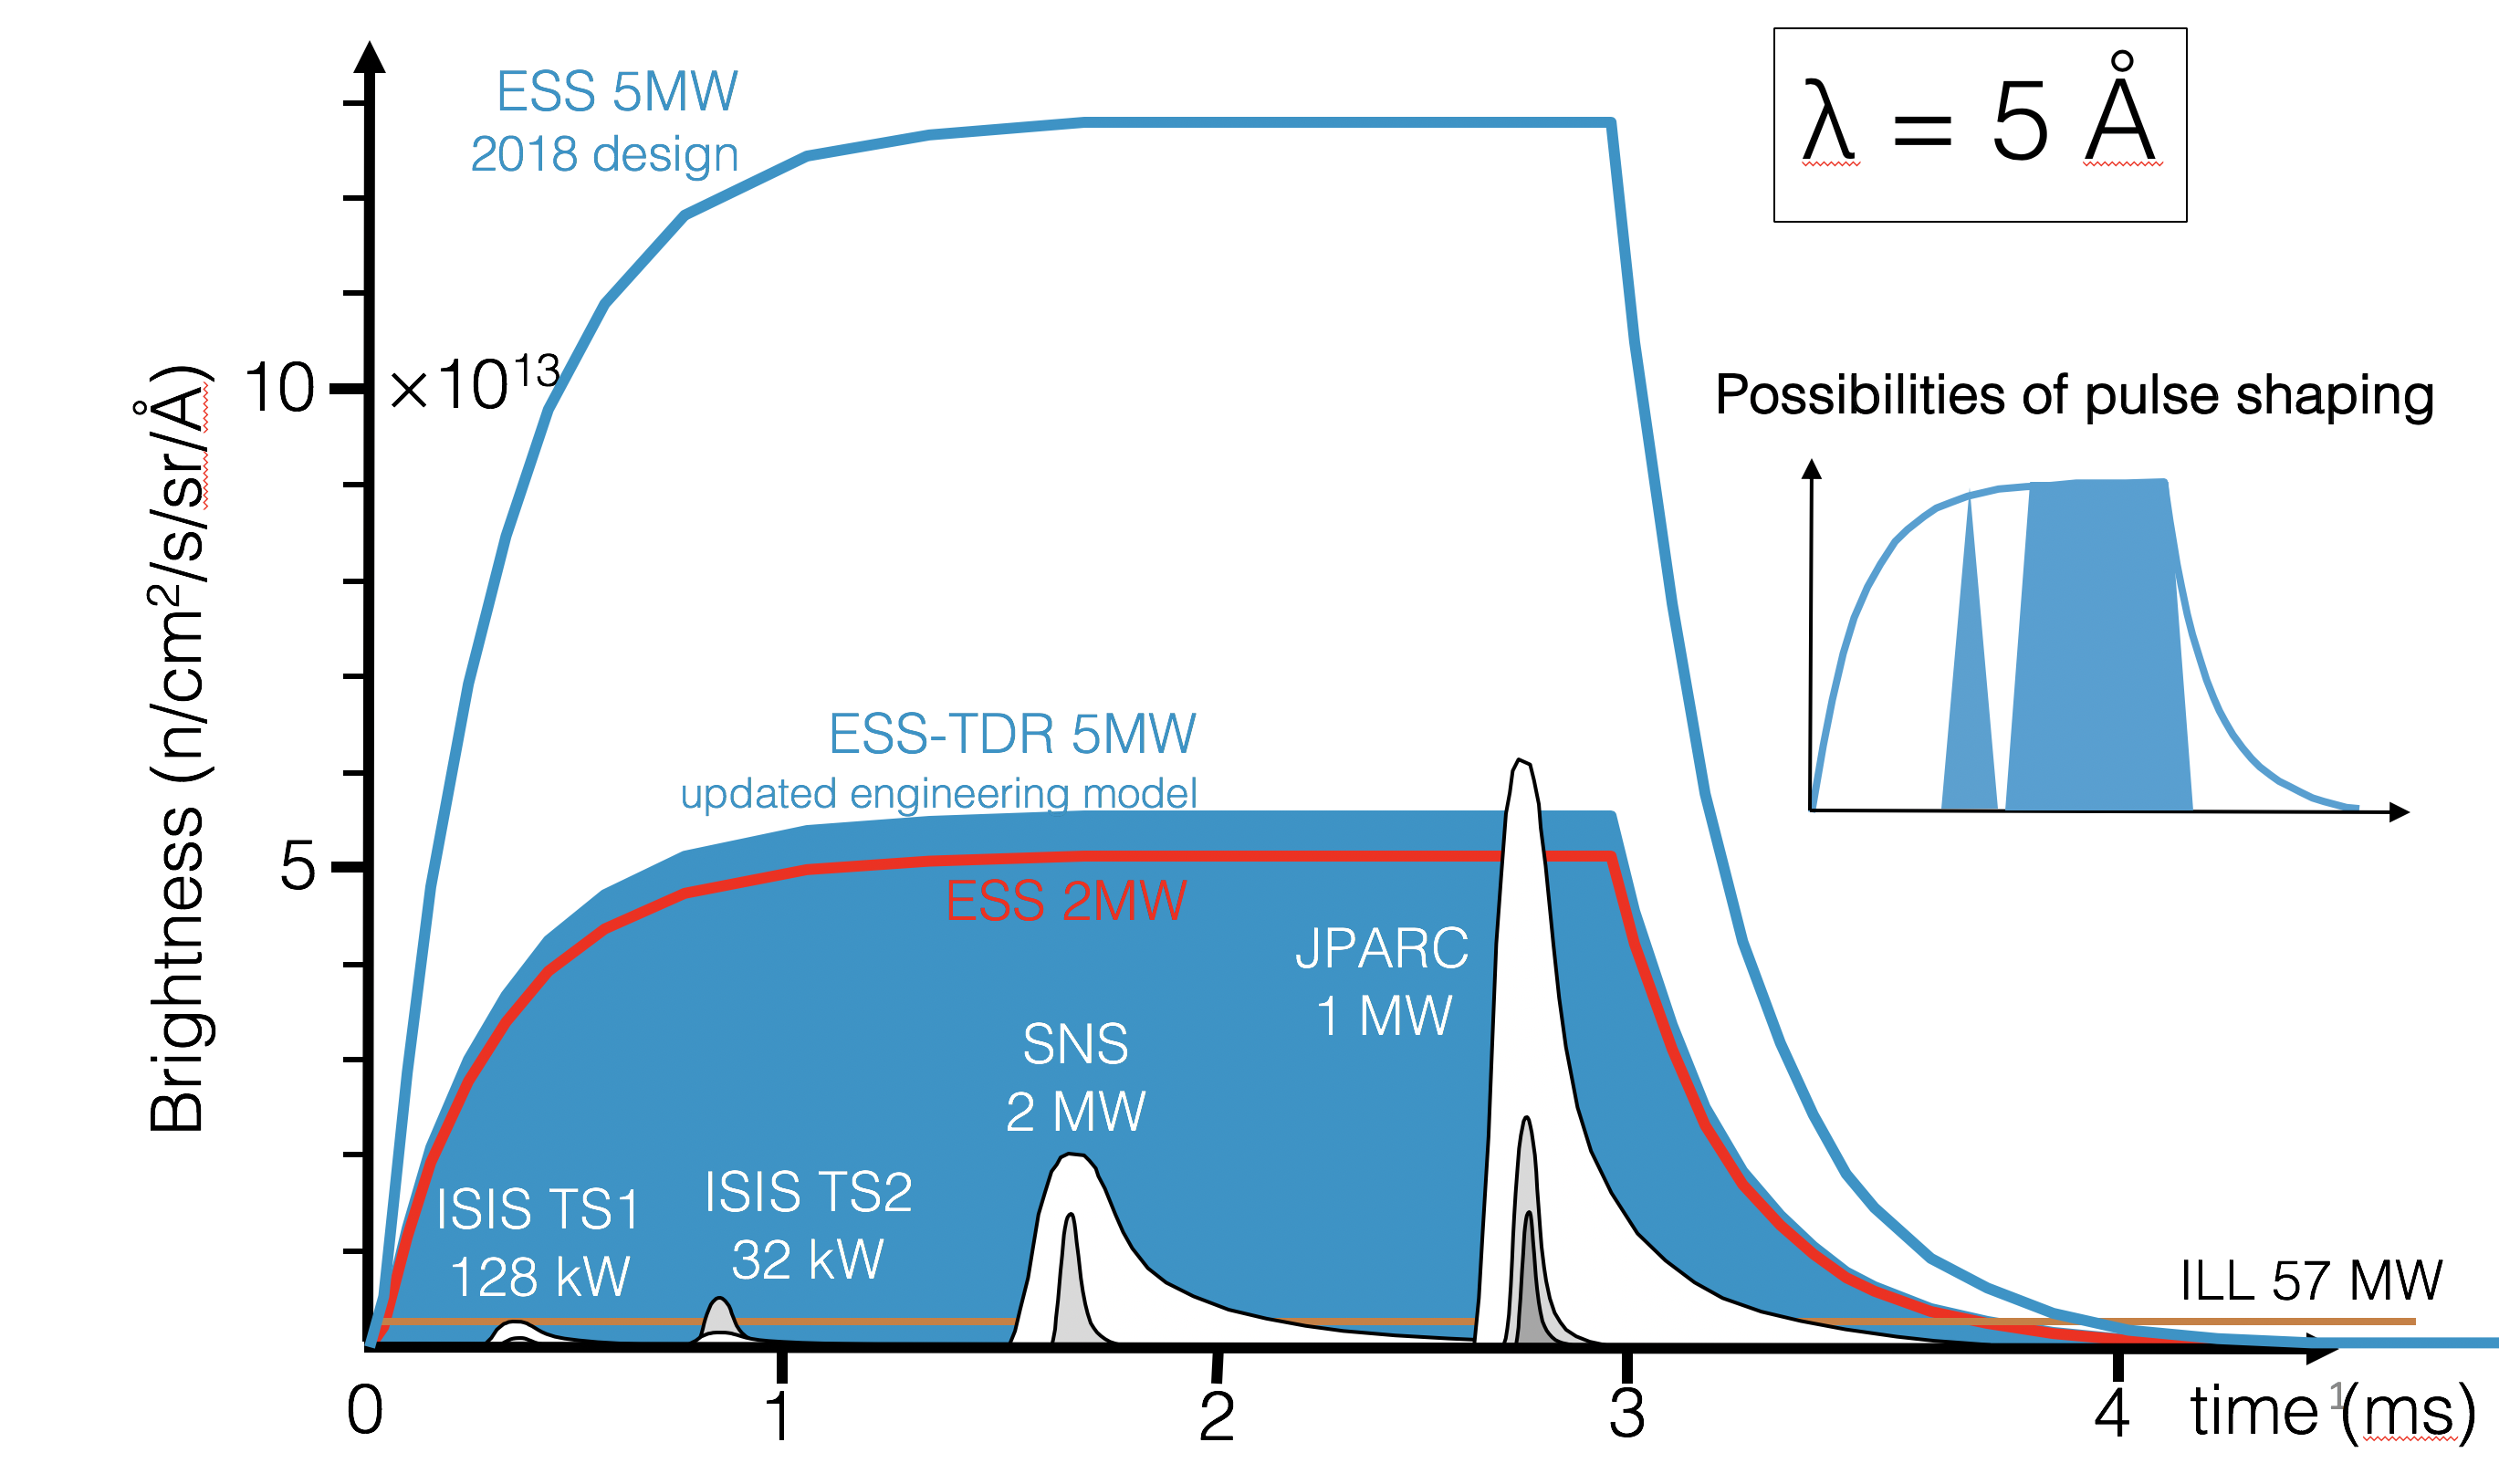
\includegraphics[width=\textwidth]{02_BeamDiag/figures/fig000_ESS_pulse}

  \end{center}
  \caption[ESS neutron source brightness compared to others existing neutron sources]{ESS neutron source brightness compared to others existing neutron sources.}
  \label{chap3:fig:ESS_pulse}
\end{figure}


  \section{ESS collaboration and ESS activities at CEA/IRFU}

  \section{Accelerator basics}

  \section{ESS accelerator}
  The proton linear accelerator (LINAC or linac) of ESS is represented synthetically in Fig. \ref{chap2:fig:ESS_acc}.
  The total length from source to target is about $600\,\mathrm{m}$ and $356\,\mathrm{m}$ are dedicated to the acceleration. The first part accelerates the beam up to $90\,\mathrm{MeV}$ by mean of conventional room temperature RF cavities. Then a cold part using superconducting cavities cooled with liquid helium is used to reach the highest energies.

  \begin{figure}[!ht]
	\begin{center}
		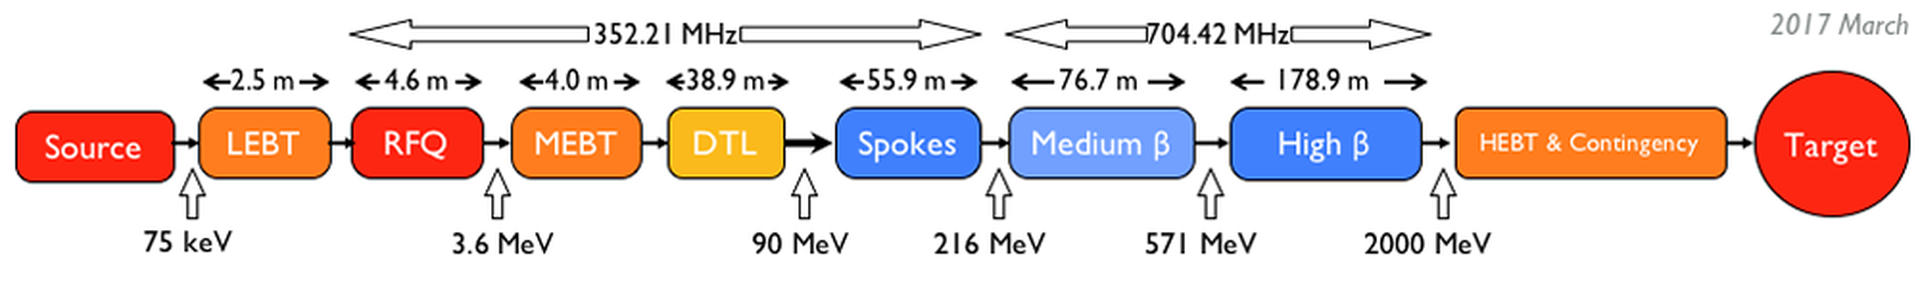
\includegraphics[width=\textwidth]{02_BeamDiag/figures/fig000_ESS_acc}
	\end{center}
	\caption[A simplified representation of the ESS linac]{A simplified representation of the ESS linac. Blue blocks represent superconducting cavities where IPMs will be installed.}
	\label{chap:}
\end{figure}


  Table \ref{chap2:tab:ess_charac} summarizes the most important characteristics of the ESS linac. The particularities of ESS compared to other sources of spallation are its very long pulse and its high current. The average beam power is 5 MW and the peak power is 125 MW, making ESS one of the most powerful proton accelerators in the world.

  \begin{table}[ht]
  \centering
  \caption[ESS nominal conditions]
  {ESS nominal conditions.}
  \label{chap2:ess_charac}
  \begin{tabular}{ll}
    \toprule
    Characteristic    & Value                  \\
    \midrule
    Energy            & $2\,\mathrm{GeV}$      \\
    Current           & $62.5\,\mathrm{mA}$    \\
    Pulse duration    & $2.86\,\mathrm{ms}$    \\
    Power             & $5\,\mathrm{MW}$       \\
    Repetition rate   & $14\,\mathrm{Hz}$      \\
    Duty cycle        & $4\,\mathrm{\%}$       \\
    Radio Frequencies & $352.21\,\mathrm{MHz}$ \\
                      & $704.42\,\mathrm{MHz}$ \\
    \bottomrule
  \end{tabular}
\end{table}

  In the present sections the role of each of the accelerator blocks is described in few words.

  \subsection{Ion source and Low Energy Beam Transport}
  The source creates the plasma that will be accelerated by the different accelerating cavities. An Electron Cyclotron Resonance (\acrshort{ecr}) sources is a type of sources particularly suitable for the production of plasma of mono specie at at high intensity \cite{nicke2012}. An ECR source is based on the superposition of a magnetic field and a RF wave. In a magnetic field the electrons orbit around the magnetic field lines with a frequency defined by:
  \begin{equation}
    \omega_{e} = \frac{eB}{m_{e}}
  \end{equation}
  By injecting a powerful RF wave of the same frequency, the electrons will enter into resonance and reach sufficient energy to ionize the medium and create a plasma. In an ECR source the plasma is confined by the magnetic field. Then, a series of electrodes placed at very high potential extract the plasma from the confinement chamber. At the source output, the beam has an energy close to $100\,\mathrm{keV}$.

  At low energies the plasma has a strong space charge and is therefore very divergent. The low energy beam transport line (\acrshort{lebt}) contains the space charge by using usually solenoids, and optimize the injection of the plasma into the first accelerating element.
  Fig. outlines the source and the LEBT of ESS. An iris allows to finely adjust the beam current in and a faraday cage is able to completely stop the beam. This line also contains diagnostics that check the quality of the beam before the injection in RFQ. The \acrshort{infn} Catania was in charge of the design and production of the source and the LEBT. CEA/IRFU was involved in two diagnostics: the Doppler Shift Unit \cite{Thomas:IPAC2017-MOPVA037} and the Emittance Meter\cite{Tuske:IPAC2017-MOPAB023}. The source was delivered to ESS and commissioned in 2018.
  
  \begin{figure}[!ht]
	\begin{center}
		\includegraphics[width=\textwidth]{example-image-a}
	\end{center}
	\caption[]{}
	\label{chap:}
\end{figure}


  \subsection{Radio Frequency Quadrupole}
  The principle of the Radio Frequency Quadrupole (RFQ) was imagined in the 1970s in Russia by Kapchinskiy and Tepliakov. The method has quickly become popular and indispensable in very intense accelerators since it still the most efficient method of acceleration at low energies.

  At these energies, the space charge is so high that the beam divergence is enormous and must be compensated. An RFQ behaves as a sequence of focusing and defocusing elements that can contain the space charge. RF waves are propagated on four poles (usually vanes or rods) with opposite amplitude between each pole. The RF variation allows to successively focus in one direction (and defocus in the other direction). A mechanical modulation of the vanes introduces a longitudinal electric field that will accelerate the particles. In concrete terms, an RFQ:
  \begin{itemize}
    \item contains and focuses the beam.
    \item accelerates the particles
    \item structures the beam into small bunches
  \end{itemize}

  \begin{figure}[!ht]
  \centering
  \begin{subfigure}[t]{0.3\textwidth}
    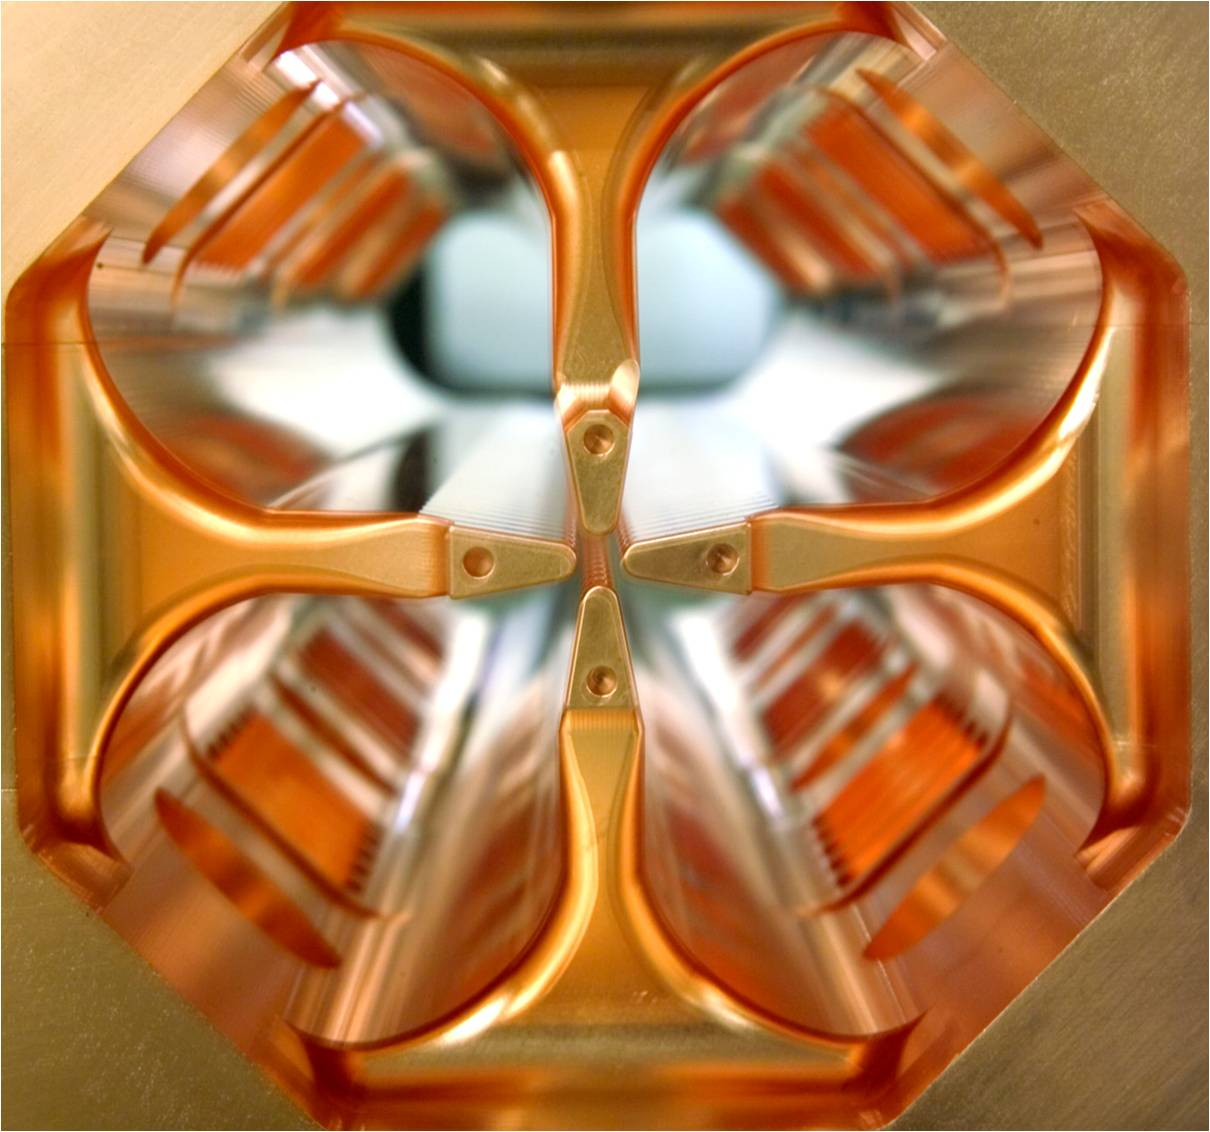
\includegraphics[width=\textwidth]{02_BeamDiag/figures/fig000_RFQ_c}
    \caption[The four copper vanes of a RFQ]{The four copper vanes (poles) of a RFQ.}
    \label{chap2:fig:RFQ_c}
  \end{subfigure}
  ~
  \begin{subfigure}[t]{.3\textwidth}
    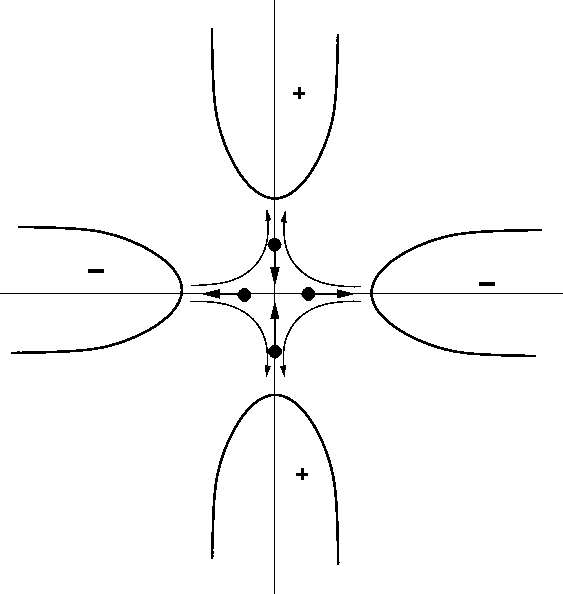
\includegraphics[width=\textwidth]{02_BeamDiag/figures/fig000_RFQ_a}
    \caption{Cut view of the transverse field.}
    \label{chap2:fig:RFQ_a}
  \end{subfigure}
  ~
  \begin{subfigure}[t]{0.3\textwidth}
    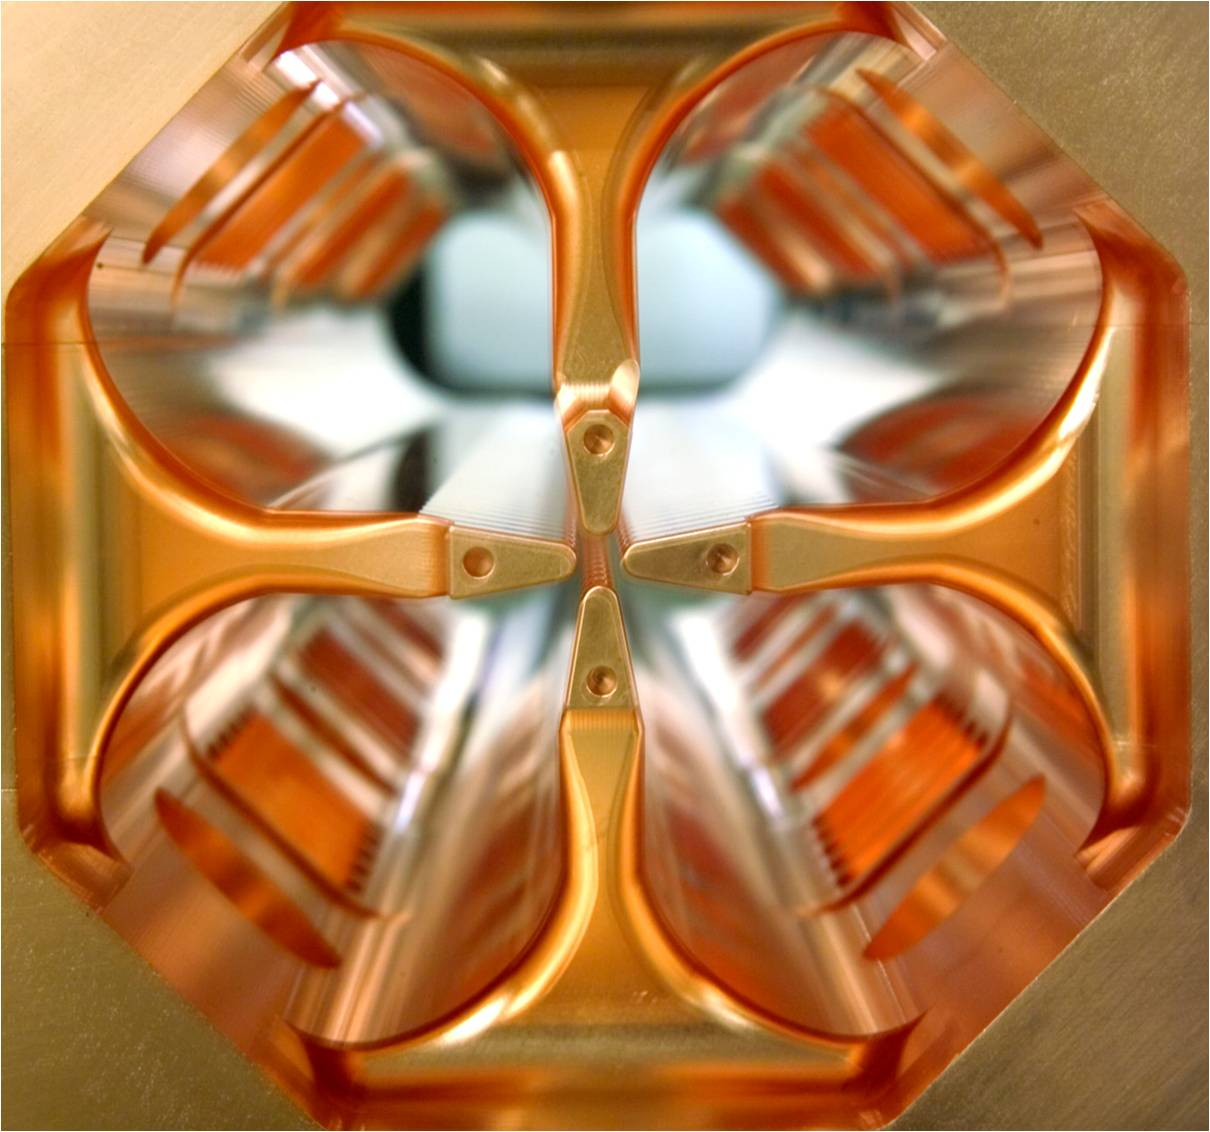
\includegraphics[width=\textwidth]{02_BeamDiag/figures/fig000_RFQ_b}
    \caption[Longitudinal modulation leading to an accelerating field]{Longitudinal modulation leading to an accelerating field \cite{Lombardi:1005049}.}
    \label{chap2:fig:RFQ_b}
  \end{subfigure}

  \caption[An RFQ structure bunches, focuses and accelerates charged particles by means of four poles that modulate the RF wave.]{An RFQ structure bunches, focuses and accelerates charged particles by means of four poles that modulate the RF wave.}
  \label{chap2:fig:RFQ}
\end{figure}


  Simulations of such device are complicated required specific codes to compute the propagation of the RF waves and the transport of particles inside the RFQ \cite{Duperrier2000}. As well, the conception of this type of cavities is extremely technical, for instance the tolerance on the mechanical structures of the vanes is in the order of micrometers whereas the whole RFQ structure often exceeds meters.

  The CEA/IRFU is in charge of the construction of the ESS RFQ \cite{ChirpazIPAC2016} which accelerates the proton at the source output to $3.6\,\mathrm{MeV}$ and bunches them with a $352.21\,\mathrm{MHz}$ frequency.

  \subsection{Medium Energy Beam Transport and Drift Tube Linac}
  The medium energy beam transport (\acrshort{mebt}) is located just downstream of the RFQ and contains beam optical elements and beam diagnostics allowing beam characterization and correction. Fig. \ref{chap2:fig:MEBT} shows a block view of the MEBT and its different elements. Most diagnoses will be presented later in the chapter and a table of abbreviations is available at the end of the thesis. The MEBT has been developed by the ESS-Bilbao team.

  \begin{figure}[!ht]
	\begin{center}
		\includegraphics[width=\textwidth]{example-image-a}
	\end{center}
	\caption[]{}
	\label{chap:}
\end{figure}


  The MEBT prepare the beam for the injection in the Drift Tube Linacs (\acrshort{dtl}).
  This type of cavity, invented by Alvarez\footnote{Sometime, the structure is referred as Alvarez Drift Tube Linac}, is a cylindrical standing waves resonant structure. It uses coaxial cylinders (drift tubes) at the end of support tubes. The acceleration occurs in the gaps between two cylinders. The cylinders are also designed to shield the field for particles during the deceleration phase. The length of these drift tubes is related to the velocity of the particles and increases along the structure. Permanent quadrupole magnet are encapsulated within the coaxial cylinders allowing a  radial focussing of the beam.

  At ESS, the DTL are designed to accelerate beam form $3.62\,\mathrm{Mev}$ Mev to $90\,\mathrm{Mev}$. The ESS DTLs have similar design to the Linac4 DTLs. The DTLs are separated in five DTL tanks containing between 61 to 23 drift tubes. Fig. \ref{} presents some pictures of the ESS DTLs.

  %\begin{figure}[!ht]
	\begin{center}
		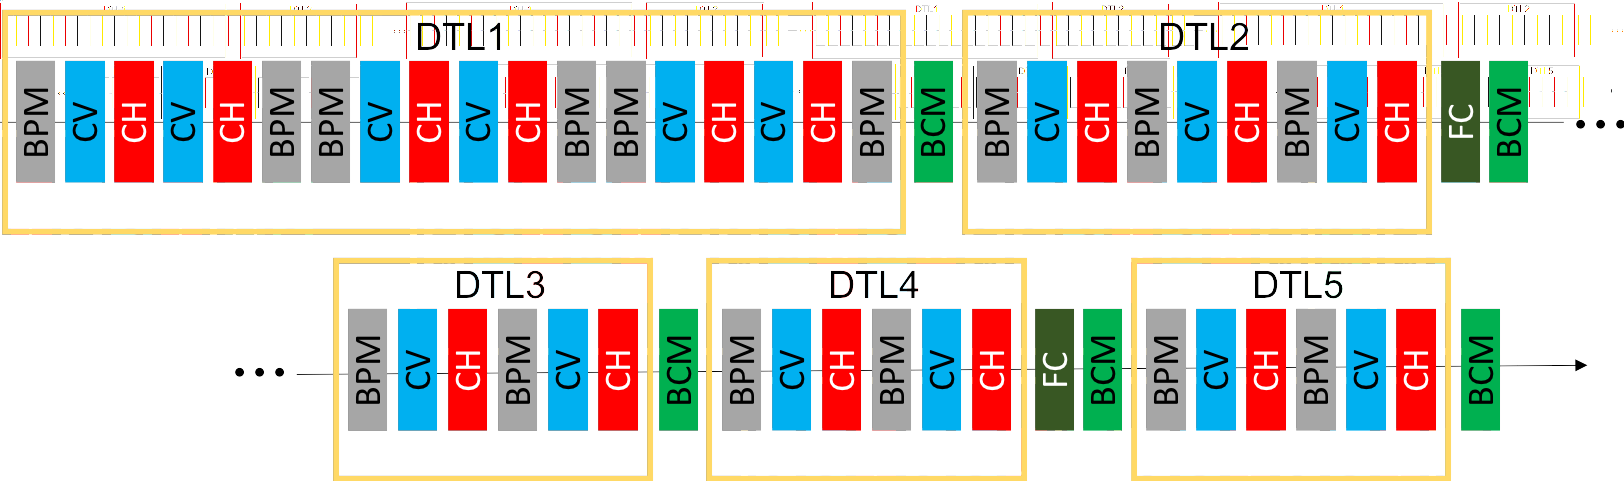
\includegraphics[width=\textwidth]{02_BeamDiag/figures/fig000_DTL}
	\end{center}
	\caption[Building blocks of the MEBT]{Building blocks of the MEBT.}
	\label{chap2:fig:DTL}
\end{figure}

  \subsection{Superconducting cavities}
  The DTL are not optimized beyond 100 MeV because the length of drift tube becomes too long. Two solutions can be considered: increase the accelerating field or increase RF frequency. However, both solutions are technically difficult to implement for long pulsed beam. Indeed, losses in the cavities become very high leading to inefficient acceleration and heating of the cavities. The use superconducting RF cavities overcomes theses issues. These superconducting cavities act as perfect conductors when the transition temperature of the superconductor is reached: $9.2\,\mathrm{K}$ for niobium.

  The cooling of these cavities is done by liquid helium at $4.13\,\mathrm{K}$ using a support tank that provides all the cooling distribution, thermal shielding, RF coupling and many more. The whole system is called cryomodule. The assembly process of the cryomodule must be done in a clean condition and particle free environment (cleanrooms). A defect on surface or a contamination lead to a loss of the superconductivity capability locally. This leads to an increase of the RF losses in this area, which in turn increases the temperature and so on. A surface defect can also increase field emission. This phenomenon occurs in all RF cavities but the supra cavities are more sensitive to the consequence of field emission.

  Our devices will be installed between two cryomodules, and therefore must be compliant with the constraints imposed by the use of superconducting cavities at ESS. The CEA/IRFU is responsible for the design and integration of medium and high beta cryomodules. Fig. \ref{chap2:fig:ESS_cryo} pictures one elliptical cryomodule.

  \begin{figure}[!ht]
	\begin{center}
		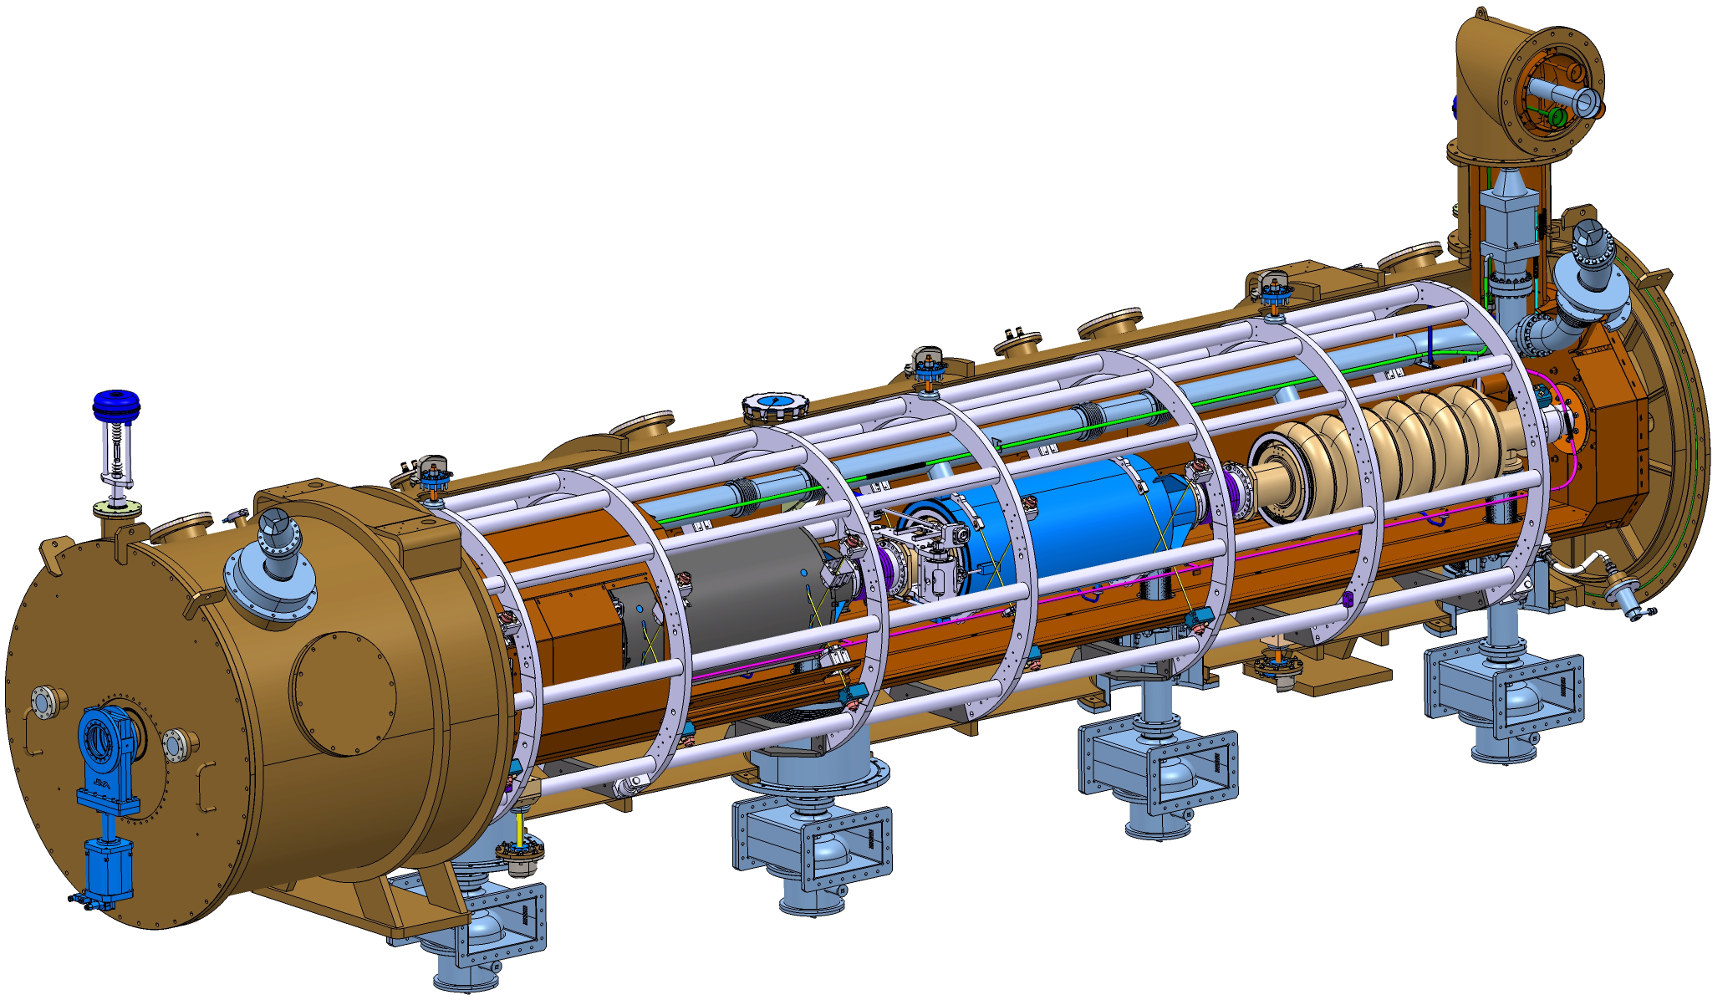
\includegraphics[width=\textwidth]{02_BeamDiag/figures/fig000_cryo_a2}
	\end{center}
	\caption[ESS medium beta elliptical cavities cryomodule]{ESS medium beta elliptical cavities cryomodule.}
	\label{chap2:fig:ESS_cryo}
\end{figure}


  \section{Transport lines and target}

  \begin{figure}[!ht]
	\begin{center}
		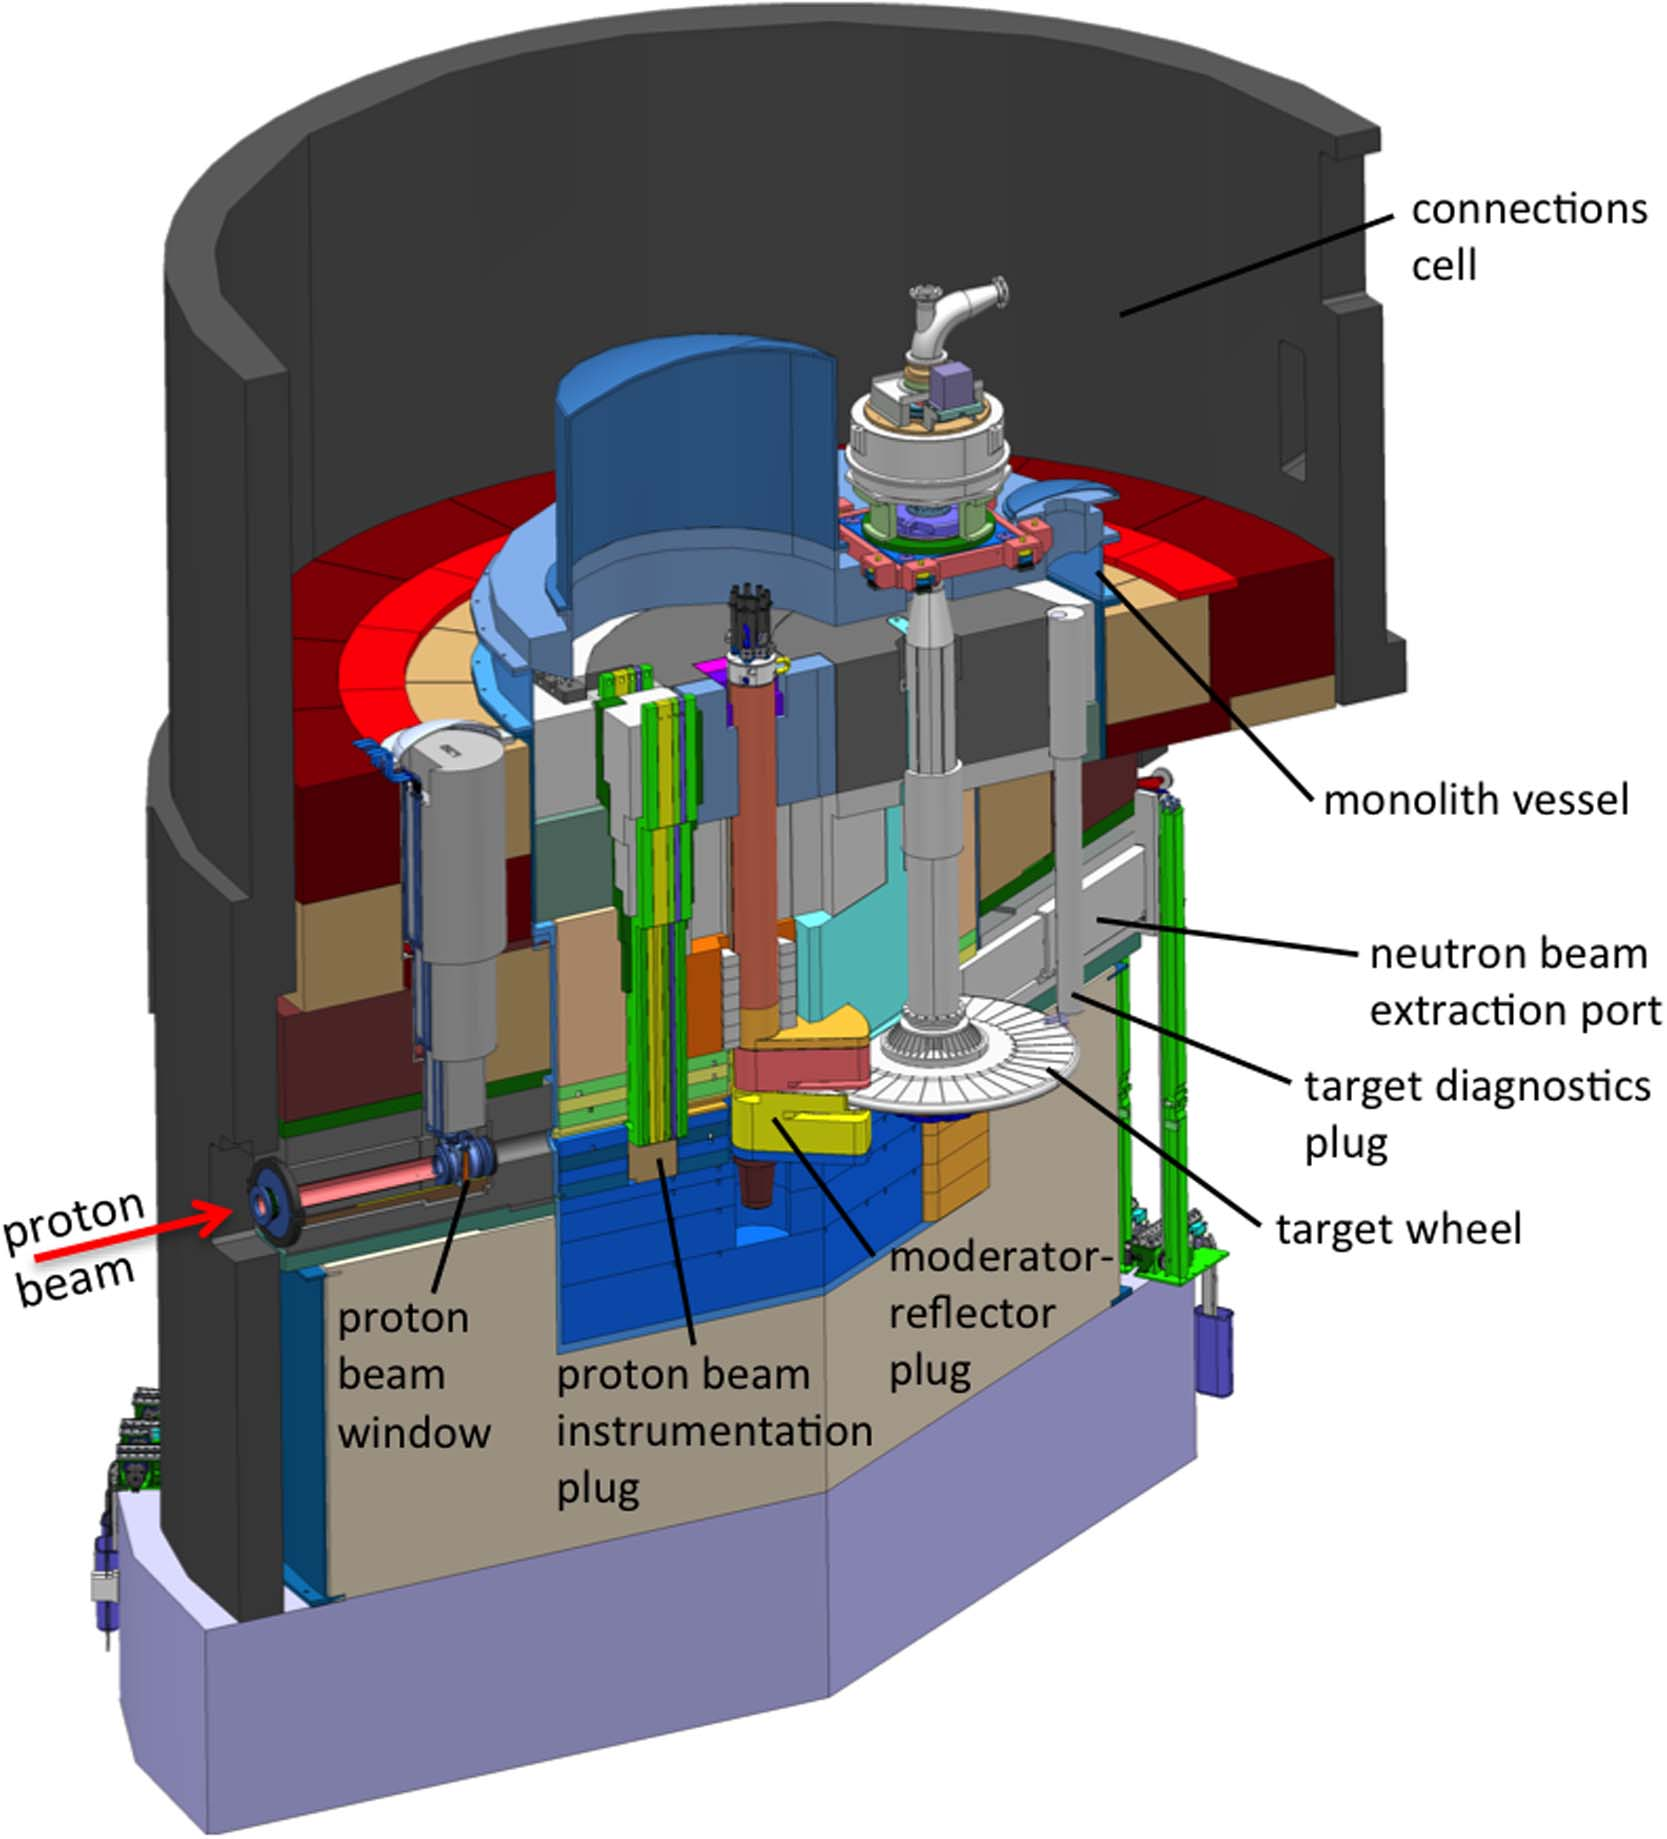
\includegraphics[width=\textwidth]{02_BeamDiag/figures/fig000_ESS_target_b}
	\end{center}
	\caption[The Tungsten target inside the monolith structure]{The Tungsten target inside the monolith structure.}
	\label{chap2:fig:target}
\end{figure}


  \section{Instruments}

  \section{Beam diagnostic overview}
  Beam diagnostics are used to ensure the proper functioning of the accelerator, the safety of persons and/or installations. They allow to measure the different beam characteristics such as current, position, energy, profile, emittance etc. For each beam characteristic several methods can be considered each of them having advantages and drawbacks. Beam diagnostics are at the crossroads of many areas of physics and electronics.

  The accelerating technologies are often complicated and quite expensive. In general, the size of the accelerator is reduced as much as possible, the space along the beam tube is often limited. The choice of diagnostics installed on a line must be done carefully according to the expectations, neglecting diagnostics may be dramatic.

  The present section briefly introduces different beam diagnostics frequently encountered on high intensity linear accelerators. Complete description of beam diagnostics can be found in books\cite{strehl2006}, Joint Universities Accelerator School \cite{juas2019} or CERN Accelerator School \cite{cas2019}.

  \subsection{Beam position monitor}
  \subsection{Beam current monitor}
  The measurement of the beam current is perhaps the most basic information for an accelerator. Beam Current Monitors (\acrshort{bcm}) detect how many beam particle are passing through specific points on the accelerator. The transmission between the different accelerating blocks can be quantified.

  The BCM rely on very different method depending on the minimum value of the currents that should be detected. In the case of ESS, the beam current can be considered as high. Two common families of methods for measuring high currents are presented in the present section.

  A Faraday cup (\acrshort{fc}) is a destructive method of current measurement. It can be seen as a beam dump, isolated from the accelerator ground, where the charges from the beam are collected by mean of a reading electronics. FC are often used in low energy parts of an accelerator (in LEBT for instance) because it can be used both as a current meter and beam dump. At high energy the size and the complexity of the FC design increase. A FC is usually placed after the iris because allowing a fine tuning of the current without having to inject it into the entire accelerator. The critical part of the design of a FC is the cooling system that must be sufficiently efficient to dissipate the thermal power deposited by the beam. Repelling or suppressors electrodes or permanent magnets must placed to avoid any parasitic current due to secondary electron emission during the impact of the beam particles.

  
  \subsection{Beam loss monitor}
  Beam Loss Monitors (\acrshort{blm}) are mandatory diagnostics in an intense particle accelerator. When particles are lost in the accelerator, they will hit and pass through the beam tube elements producing various radiations. In an accelerator, the losses are  to guarantee the safety of the installation. Indeed, when the loss rates are high, the devices around the accelerator can be severely damaged.

  BLMs are very often connected to the machine protection system (\acrshort{mps}) allowing a fast shut down of the accelerator if the losses are too high. BLMs relies on a wide range of radiation detection techniques.

  At ESS two types of BLM are foreseen. The first loss monitors is based on ionization chambers (\acrshort{icblm}) \cite{Grishin:IBIC2017-WEPWC03}. These are the most common BLM type, and icBLM are widely used at LHC \cite{HOLZER20122055}, SNS etc. In an icBLM, the losses ionize the gas in the chamber and a current is established between the electrodes. An icBLM has an high dynamic range, fast response and are cost effective.
  The second type of ESS BLM is completely new: the neutron Beam Loss Monitors (\acrshort{nblm}) \cite{Papaevangelou:HB2018-THA1WE04}.
  A nBLMs is sensitive to fast neutrons and insensitive to other radiation emitted by accelerator cavities. In fact, nBLM is a double detector based on micromegas detectors:
  \begin{itemize}
    \item A fast detector, sensitive to high losses allowing a very fast stopping of the beam.
    \item A slower detector, but more sensitive detector allowing a finely monitoring of the losses.
  \end{itemize}

  A total of 266 icBLMs, 42 slow nBLMs and 42 fast nBLMs will be installed along the accelerator.

  \subsection{Beam emittance measurements}

  \section{Invasive beam profile measurements}
  \subsection{Interceptive screen}
  An luminescent screen provides a convenient way to measure profile since this diagnostic is simple to implement. The screen is put directly on the beam path using a translator. When particles pass through the material they will deposit their energy and excite the medium. During the de-excitation process, the energy is released to photons. The intensity on the screen is proportional to the number of incident particles. Therefore, it is possible to measure the profile directly in two dimensions with one camera by tilting the screen.

  The use of this diagnostic is strongly limited by the energy and intensity of the beam. At low energies and/or high current, the power to be dissipated can be locally considerable altering the screen properties. In general, a permanent decrease of the screen yield is observed \cite{Simon:IBIC2016-MOPG79} and in some extreme cases a deterioration of the screen surface.

  A concrete use of this type of diagnosis will be briefly presented in Chapter 4 with some experimental results.

  There is another type of intrusive diagnosis based on the optical transition radiation. The setup looks similar but the process behind is totally different. When a relativistic particle is subject to sudden variation of dielectric constant, i.e. between two media, transition photons are emitted with precise angles depending to the particle, its velocity and the angle of incidence. This method is well adapted for high relativistic accelerators such as $e^{-}$ \acrshort{linac} \cite{Nolle2009,Bolzon2013}.

  \subsection{Wire scanner}
  \subsection{SEM-Grid}
  A Secondary Electron EMission grid (SEM-Grid) or harp grid is a multichannel version of the SEM WS. Several wires are taut in the same direction at several position. To avoid crosstalk due to secondary electrons, an electron repeller (wire or electrode) is often placed around the wires. A second wire plane can also be placed in the other transverse direction. Therefore, the profile is measured in one shot in the two transverse directions without moving the device during the measurement. By using several SEM-grid successively the measurement of the transverse emittance is possible.

  However, the readout electronics is more complex because the number of wires is multiplied. The number of wire must be choose according to the requirement on the resolution on beam size and position. The wires must meet the same constraints as the wire scanner. The system is not necessarily more robust because if one wire breaks it may short circuit the other wires nearby.

  \section{Non-invasive beam profile measurements}
  \subsection{Laser wire profiler}
  \subsection{Beam induced fluorescence profiler}
  \section{Ionization Profile Monitor and summary}
  The fluorescence profiler can not work when

  The first use of IPMs dates back to the 1960s \cite{DeLuc1969}.
  In the 90s, the raise of the MicroChannel Plates have permitted to measure profiles \cite{Krider1989,Wittenburg1992} in more critical working conditions.
  The IPM method is now mature and used in several installations \cite{Satou2006,Giacomini2011,Morris2011,egberts2012}.

  Recently, the interest in semiconductor detectors has grown \cite{Storey2015} and first results looks promising \cite{Storey2017}.

  The different technologies of detection, presented just before, have been reviewed in order to select the most efficient one with respect to the ESS requirements. 

  \begin{figure}[!ht]
  \centering
  \begin{subfigure}[t]{0.45\textwidth}
    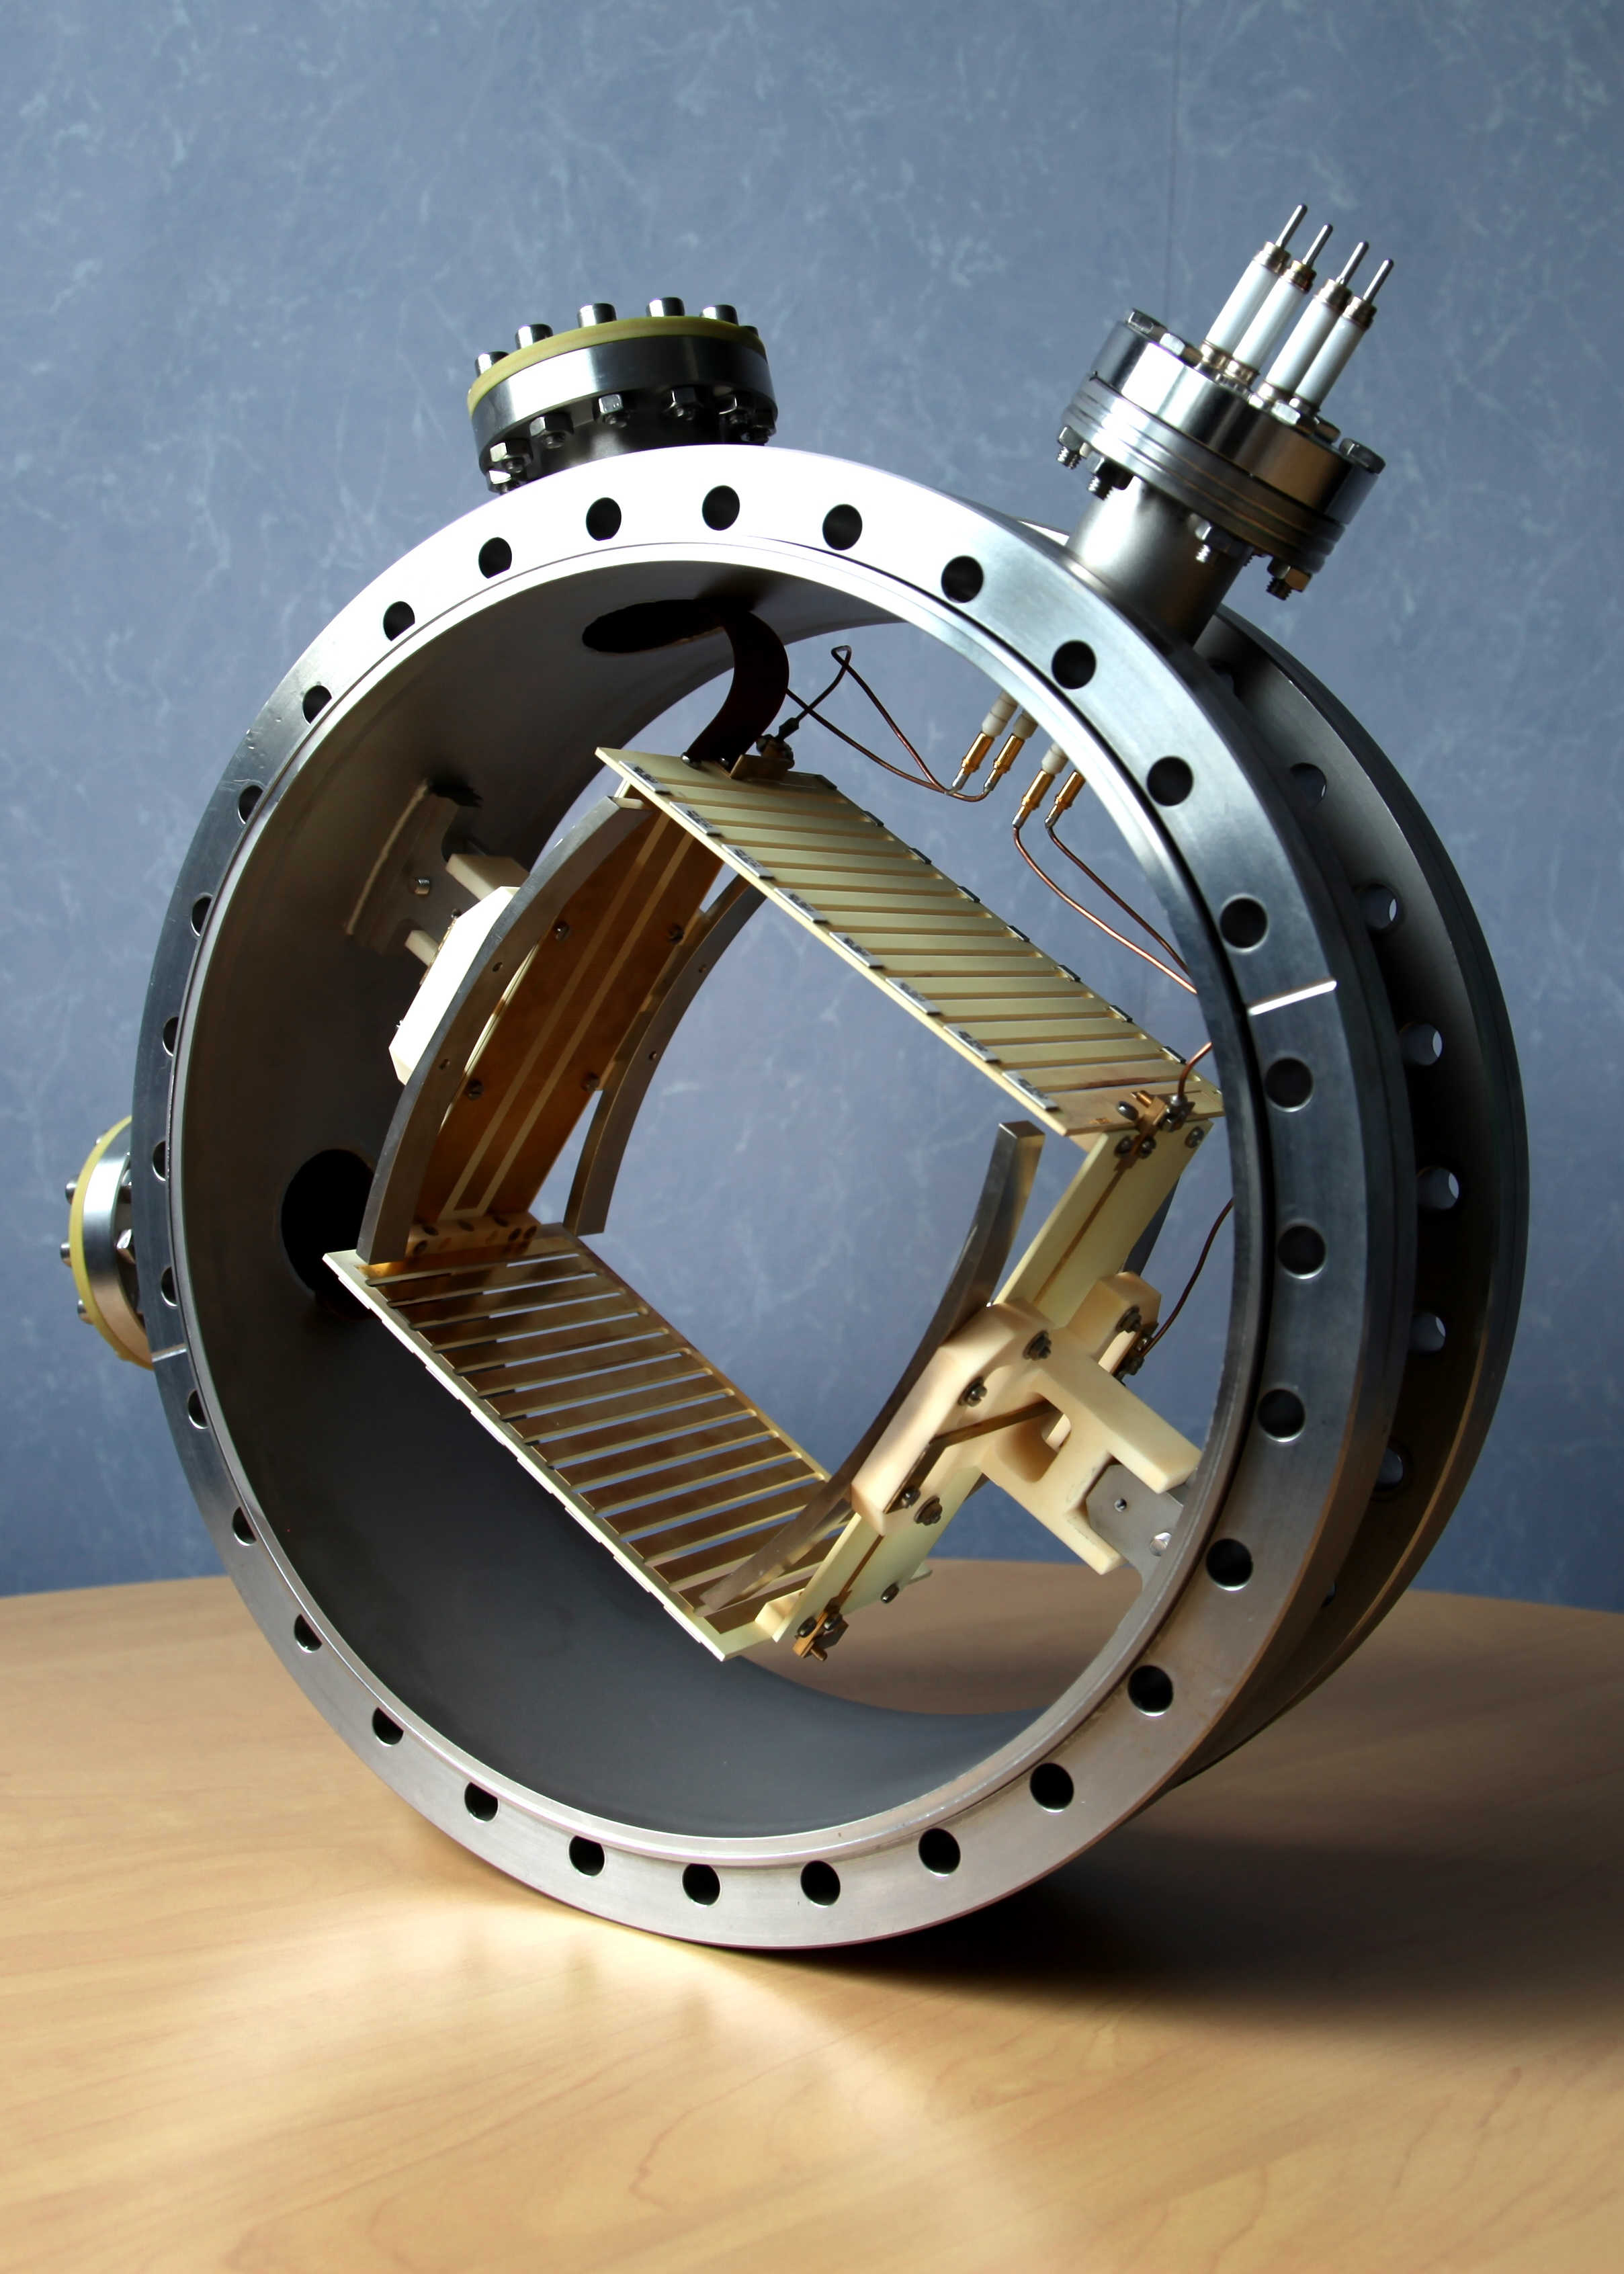
\includegraphics[width=\textwidth]{02_BeamDiag/figures/fig000_IPM_1}
    \caption[One of the IPM at IFMIF]{One of the IPM at IFMIF \cite{egberts2012}.}
    \label{}
  \end{subfigure}
  ~
  \begin{subfigure}[t]{0.45\textwidth}
    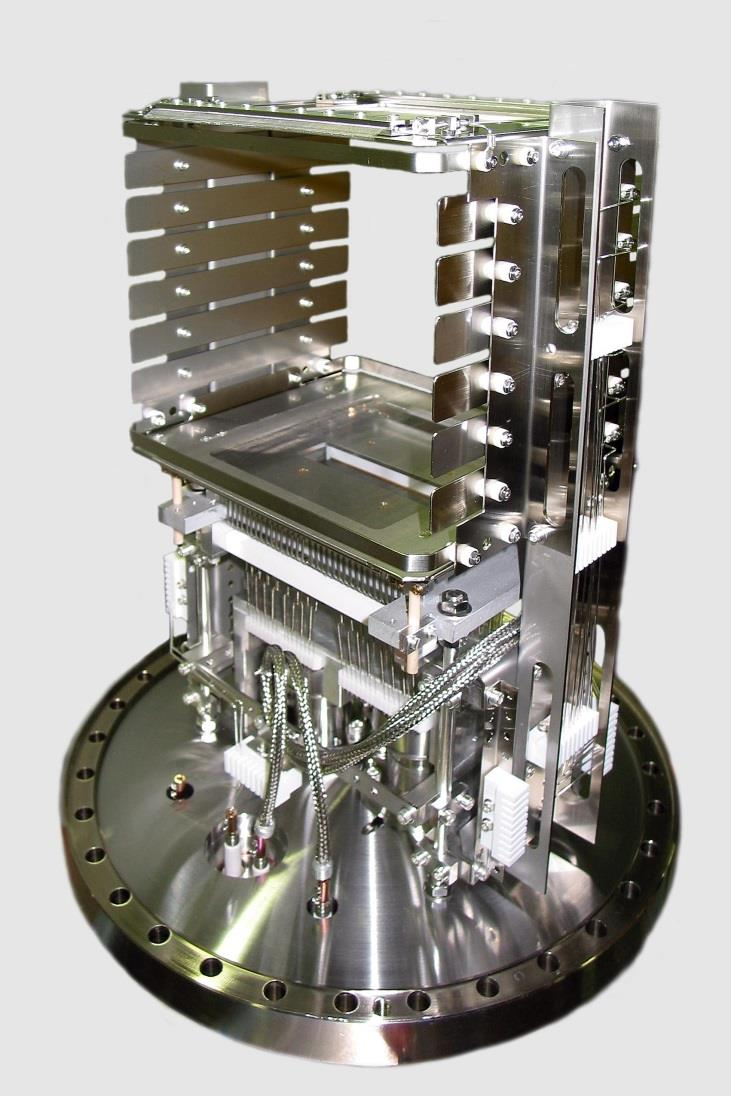
\includegraphics[width=\textwidth]{02_BeamDiag/figures/fig000_IPM_2}
    \caption[One of the IPM at GSI]{One of the IPM at GSI \cite{ForkJUAS}.}
    \label{}
  \end{subfigure}
  
  \begin{subfigure}[t]{1\textwidth}
    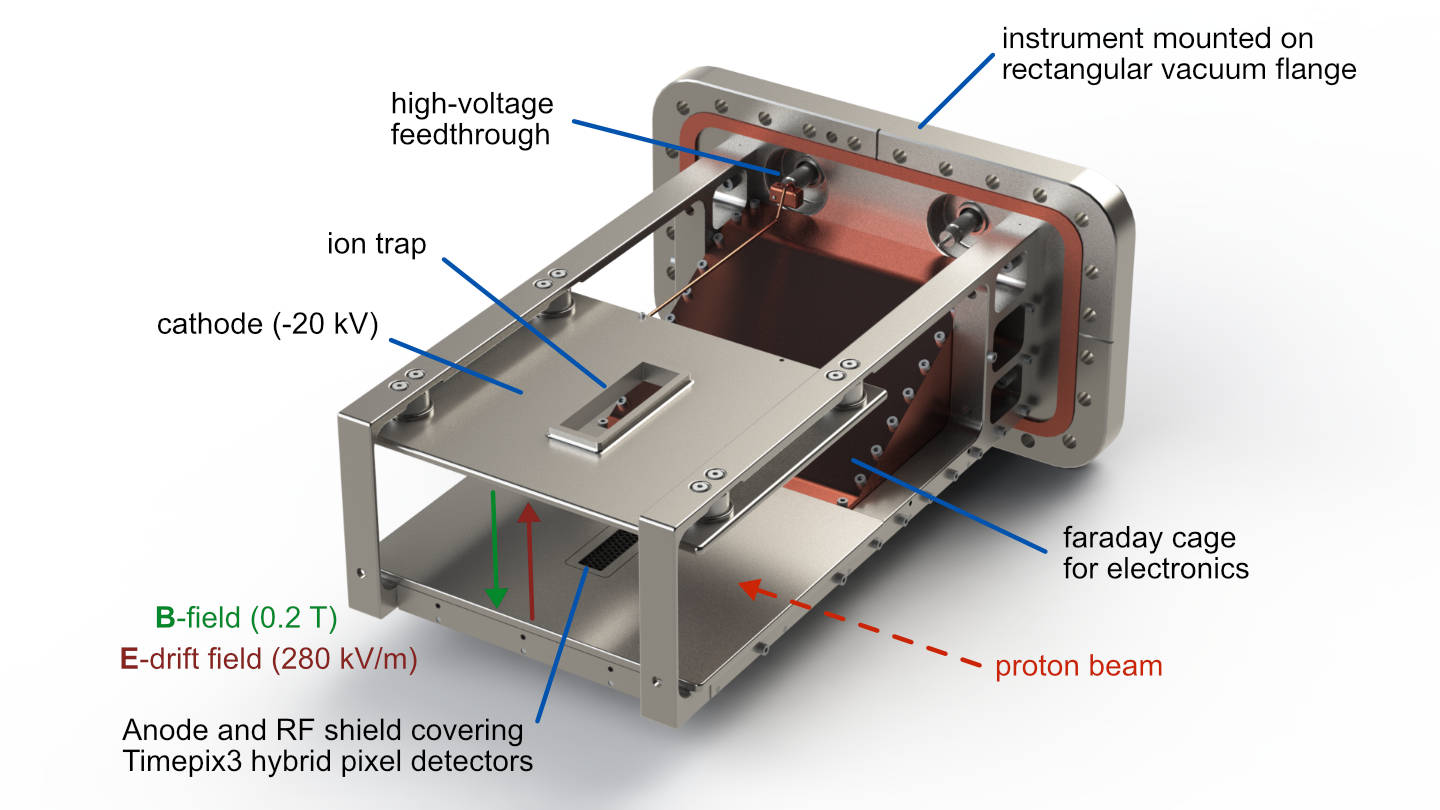
\includegraphics[width=\textwidth]{02_BeamDiag/figures/fig000_IPM_3}
    \caption[The future IPM for the PS]{The future IPM for the PS \cite{Storey2017}.}
    \label{}
  \end{subfigure}
  \caption[Three different implementations of IPMs on three different accelerators]{Three different implementations of IPMs on three different accelerators.}
  \label{chap2:fig:IPM_3}
\end{figure}


  \cleardoublepage
  \section*{Bibliography}
  \addcontentsline{toc}{section}{Bibliography}
  \label{ch2:bib}
  \printbibliography[heading=subbibliography]

\end{refsection}